%%==================================================
%% chapter03.tex for SJTU Course Design Thesis
%% based on CASthesis, SJTU master thesis
%% modified by icetiny@gmail.com
%% version: 0.3a
%% Encoding: UTF-8
%% last update: Dec 5th, 2010
%%==================================================

% \bibliographystyle{sjtu2} %[此处用于每章都生产参考文献]
\chapter{系统功能设计}
\label{chap:functionintro} 
	本章起到一个功能说明书的作用,将抛开底层的硬件和具体的软件实现,面向普通用户,介绍本系统的主要功能、工作流程,以及设置界面的使用方法。本章也作为下一章软件设计的先导,软件设计都是围绕着以下功能的实现而进行的。
	
	合理的硬件设计也是以下功能实现的重要基础。
\section{信号灯交替流程}
	红黄绿三色信号灯按照图\ref{fig:lightbullflow}所示的工作顺序交替闪亮。由于相交的两条路交通状况可能相差很大,其红灯持续时间是不同的。两个红灯时间T1和T2可以分别设置\footnote{下文将称这两个参数为亮灯时间参数},黄灯时间默认为3秒。由图可见一个亮灯循环只需要两个独立参数(T1和T2)就可以确定,绿灯时间比相应红灯时间短3秒。
	\begin{figure}[!tbh]
      \centering
      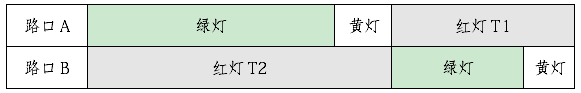
\includegraphics[width=0.9\textwidth]{chap3/lightbullflow.png}
      \bicaption[fig:lightbullflow]{亮灯顺序循环图}{亮灯顺序循环图}{Fig}{Signal light changing pattern}
    \end{figure}
    
	各个路口均悬挂有倒计时显示器,两组相对的路口显示内容分别相同。倒计时的内容为当前亮的灯将要持续的时间。当显示完\textbf{00}之后,灯的状态改变,倒计时显示屏也重新开始计数。 
	
\section{可调的亮灯时间}
所谓亮灯时间的可调性,就是指图\ref{fig:lightbullflow}中的循环参数T1和T2是可变的,这是为了适应不同的交通状况,车流量大时缓解拥堵,车流量小时减少等待。调节亮灯时间的方式有以下三种。
\subsection{预置数据表调节} 在单片机的ROM中预先存放了一数据表,一天中的每小时\footnote{一天中划分为24个时间段,从0到23,分别对应一天中的第一到第24个小时。}都有存储了两个数据在表中,分别代表A路口和B路口的红灯时间。则此表格共包含48个数据。单片机会根据当前的时间段\footnote{单片机复位后,用户可通过键盘设定初始时区为当前时间段,如图\ref{fig:keysetflow},之后单片机即从此时区开始自动累加},自动切换亮灯时间。
\subsection{用户自定义亮灯时间} 本系统还提供了一人机界面(包括5个按键和2位数显屏)供用户随时调节亮灯时间。用户可以调节任一时间段的亮灯时间,也可以重新定义当前所处的时间段。若用户调节了当前时间段的亮灯时间,则在当前红灯倒计时变为0后立即生效。\ref{sec:functionkeyboard}节会详细介绍该方式的使用方法。

时间参数存储在RAM中,单片机复位后会全部清零。用户定义的时间参数优先级比内置参数表高。
\subsection{双机通信调节} 单片机系统中留出了接口,上位机可以通过串行接口向单片机发出指令,直接改变当前时间段的亮灯时间参数。上位机可以是自动监控车流量的单片机,也可以是交通管理网络中的计算机。这种调节方式和通过键盘的调节方式,后设置的参数会覆盖之前覆盖的参数,所以它们的优先级是一致的。

\section{键盘屏显接口使用方法} \label{sec:functionkeyboard}
用户通过键盘可以实现两个功能。
\begin{enumerate}
\item 设定任一时段两路口的红灯时间参数,该参数存入RAM中。
\item 当用户设定的数据为两个00,则更改目前的时间区段为用户设定的值,这一功能可用于在单片机复位后初始化当前时区。
\end{enumerate}
在设定过程中,数字显示的相应位会闪烁,提示用户目前正在操作的位的位置。
\subsection{键位定义} \label{sec:keydefination}
		表\ref{tab:keydef}详细列出了各个按键的定义,了解了这张表基本就可以尝试操作了。但是由于屏显只有两位数码管,刚开始也许还会有些费解,还需要参考\ref{sec:keysetflow}节给出的一个完整的设置流程图。
		\begin{table}[!htpb]
      	\centering
      	\bicaption[tab:keydef]{键位定义}{键位定义}{Table}{keyboard defination}
      	\begin{tabular}{lcc|p{0.6\textwidth}} \toprule
        \multicolumn{2}{c}{键名} & 端口 & \multicolumn{1}{c}{功能} \\ \midrule
        开关 &on/off & p2.3 & 开关显示屏。开屏则首先显示当前时间段代码。关屏则重置键盘接口,清空所有寄存器。\\ \hline
        确认键&ok & p2.4 & 确认当前选择,并前进到下一选择界面\\ \hline
        选位键&<> & p2.5 &切换选择高低位。在设定数码时,用于在个位十位间切换,被选择的位会闪烁。设定时间段时,该键不起作用。\\ \hline
        加一键& + & p2.6 &使屏显的内容加一。在红灯时间调节状态下,对闪烁的位加一。若超出最大值,则变为最小值。\\ \hline
        减一键& -  & p2.7 &使屏显的内容减一。在红灯时间调节状态下,对闪烁的位减一。若小于最小值,则变为最大值。\\ 
				 \bottomrule
      	\end{tabular}
		\end{table}
\subsection{键盘设定操作流程}  \label{sec:keysetflow}
图\ref{fig:keysetflow} 是键盘相关的完整流程图。从图中可以明确看到,通过键盘设定可以完成两个功能。

需要补充的一点是,在成功设置某一时段的时间参数后,程序将检查设置的是否就是当前时段,如果是的话,会重新载入该时间常数。故更改会在当前红灯倒计时完毕后立即生效。
\begin{figure}[!tbhp]
      \centering
      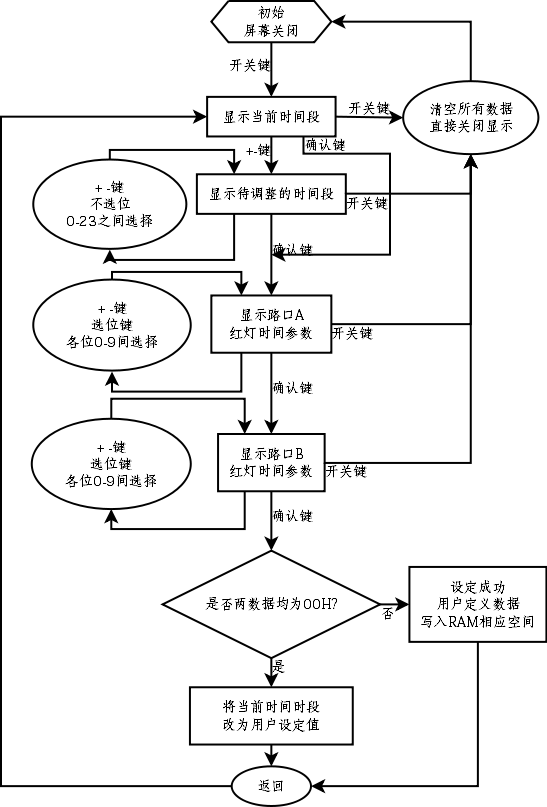
\includegraphics[width=0.85\textwidth]{chap3/keysetflow.png}
      \bicaption[fig:keysetflow]{键盘操作流程图}{键盘操作流程图}{Fig}{keyboard control flow figure}
    \end{figure}
\subsection{强壮性设计}
如果用户向信号灯系统定义了两个0为时间参数,显然这样的定义是没有意义的,通过软件已经将这样的输入转换为对当前时间段的重定义。本节就将讨论用户对用户各种输入数据的处理。

因为黄灯时间需要持续三秒,所以红灯时间必须大于3秒,任何小于三秒的定义也是无效的。
	\begin{table}[!htpb]
      	\centering
      	\bicaption[tab:keyresetmap]{键盘输入处理}{键盘输入处理}{Table}{keyboard input interpretation}
      	\begin{tabular}{c c |c c} \toprule
        \multicolumn{2}{c|}{用户输入}  &  \multicolumn{2}{c}{\multirow{2}*{相应处理}}  \\ \cmidrule(lr){1-2}   
        T1 & T2 \\ \cmidrule(lr){1-1}  \cmidrule(lr){2-2} \cmidrule(lr){3-4} 
        0 & 0 & \multicolumn{2}{c}{设置当前时间段} \\
        $\ge 0, <3$ & $\ge 0, <3$  & \multicolumn{2}{c}{无效输入,不操作}\\
        $\ge 0, <3$  & 有效输入T2 & T2 写入A路口对应RAM & T2 写入A路口对应RAM \\
        有效输入T1 & $\ge 0, <3$ & 写入T1 & 写入T1 \\
        有效输入T1 & 有效输入T2	& 写入T1 & 写入T2 \\ \bottomrule
      	\end{tabular}
		\end{table}

表\ref{tab:keyresetmap}列出了软件中对于各种输入情况的处理。由表可见,程序会自动消除用户的错误输入。默认的修正原则是:如果两个数据都错误则抛弃;如果其中有一个数据有效,则另一个路口的时间参数取相同的值。

\section{闯红灯拍照功能}
本系统还具有对闯红灯的车辆拍照的功能。需要说明的是,四个路口分别布置了地感线圈,只有在该路为红灯状态时,地感线圈发出的信号才有效。系统可以响应两个相对的路口同时闯红灯的状况,虽然这种情况的几率并不大。

\section{仍待加入的功能}
待完成